\section{Register description}
\regover{
{\hyperref[audac-audac-0]{audac\_0}}&Clock control register
\\
\hline
{\hyperref[audac-audac-status]{audac\_status}}&Status register
\\
\hline
{\hyperref[audac-audac-s0]{audac\_s0}}&Volume control register 1
\\
\hline
{\hyperref[audac-audac-s0-misc]{audac\_s0\_misc}}&Volume control register 2
\\
\hline
{\hyperref[audac-audac-zd-0]{audac\_zd\_0}}&zero detect control register
\\
\hline
{\hyperref[audac-audac-1]{audac\_1}}&
\\
\hline
{\hyperref[audac-audac-fifo-ctrl]{audac\_fifo\_ctrl}}&fifo control register 
\\
\hline
{\hyperref[audac-audac-fifo-status]{audac\_fifo\_status}}&fifo status register 
\\
\hline
{\hyperref[audac-audac-fifo-data]{audac\_fifo\_data}}&fifo data register 
\\
\hline
}

\subsection{audac\_0}
\label{audac-audac-0}
Address:0x20055000
 \begin{figure}[H]
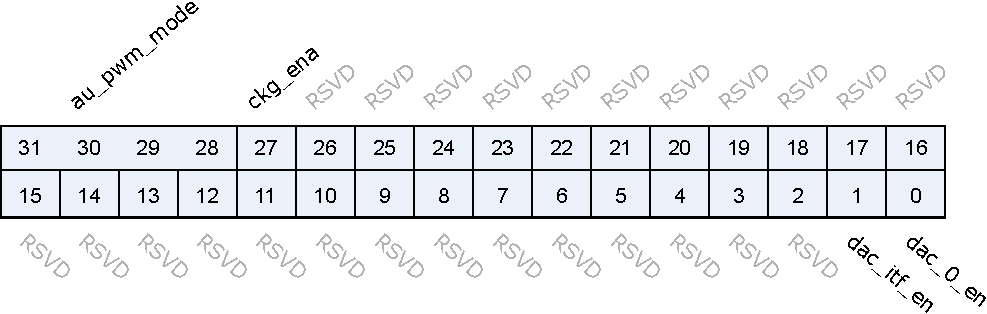
\includegraphics{audac_audac_0.pdf}
\end{figure}

\regdes{31:28&au\_pwm\_mode&r/w&4'd0&pwm output mode,rang 0 ~ 6: \par 0:8KHz, 1:16KHz, 2:32KHz, 3:24KHz, 4:48KHz, 5:22.05KHz, 6:44.1KHz \par gpdac output mode,rang 9 ~ 14: \par 9:16KHz, 10:32KHz, 11:24KHz, 12:48KHz, 13:22.05KHz, 14:44.1KHz,
\\\hline
27&ckg\_ena&r/w&1&enabl eclock gen\\\hline
26:2&RSVD& & & \\\hline
1&dac\_itf\_en&r/w&0&enable dac to audio dma interface\\\hline
0&dac\_0\_en&r/w&0&enable dac ch0\\\hline

}
\subsection{audac\_status}
\label{audac-audac-status}
Address:0x20055004
 \begin{figure}[H]
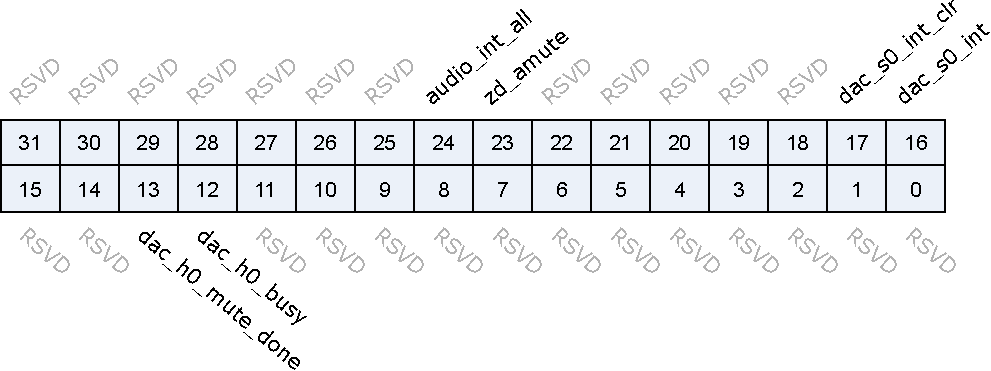
\includegraphics{audac_audac_status.pdf}
\end{figure}

\regdes{31:25&RSVD& & & \\\hline
24&audio\_int\_all&r&0&mute signal to analog\\\hline
23&zd\_amute&r&0&zero detect signal to analog\\\hline
22:18&RSVD& & & \\\hline
17&dac\_s0\_int\_clr&r/w&0&clear and close interrupt\\\hline
16&dac\_s0\_int&r&0&mute done interrupt status\\\hline
15:14&RSVD& & & \\\hline
13&dac\_h0\_mute\_done&r&1&dvga mute done\\\hline
12&dac\_h0\_busy&r&0&dvga busy\\\hline
11:0&RSVD& & & \\\hline

}
\subsection{audac\_s0}
\label{audac-audac-s0}
Address:0x20055008
 \begin{figure}[H]
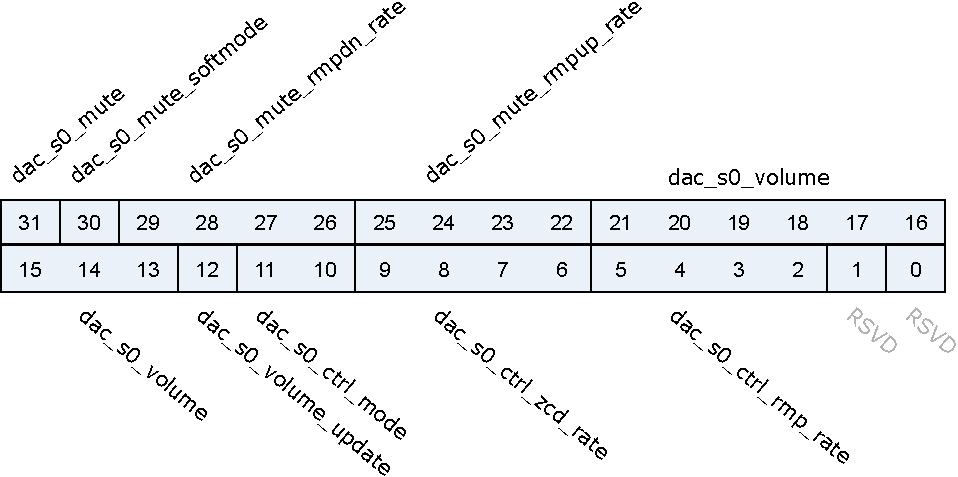
\includegraphics{audac_audac_s0.pdf}
\end{figure}

\regdes{31&dac\_s0\_mute&r/w&0&dac dpga ch0 sw volume control \par 1:mute
\\\hline
30&dac\_s0\_mute\_softmode&r/w&1&0:mute directly, 1:mute with ramp down\\\hline
29:26&dac\_s0\_mute\_rmpdn\_rate&r/w&4'd6&mute ramp down rate:  \par 0:2 fs sample \par 1:4 fs sample \par 2:8 fs sample \par 3:16 fs sample \par 4:32 fs sample \par 5:64 fs sample \par 6:128 fs sample \par 7:256 fs sample \par 8:512 fs sample \par 9:1024 fs sample \par 8:2048 fs sample \par 
\\\hline
25:22&dac\_s0\_mute\_rmpup\_rate&r/w&4'd0&mute ramp up rate \par 0:2 fs sample  \par 1:4 fs sample \par 2:8 fs sample \par 3:16 fs sample \par 4:32 fs sample \par 5:64 fs sample \par 6:128 fs sample \par 7:256 fs sample \par 8:512 fs sample \par 9:1024 fs sample \par 8:2048 fs sample
\\\hline
21:13&dac\_s0\_volume&r/w&9'd0&volume s9.1, -95.5dB ~ +18dB in 0.5dB step\\\hline
12&dac\_s0\_volume\_update&r/w&0&enable volume update\\\hline
11:10&dac\_s0\_ctrl\_mode&r/w&2'd2&0:direct force volume, 1:update volume at zero crossing, 2:update volume with ramp\\\hline
9:6&dac\_s0\_ctrl\_zcd\_rate&r/w&4'd2&zero crossing rate \par 0:2 fs sample  \par 1:4 fs sample \par 2:8 fs sample \par 3:16 fs sample \par 4:32 fs sample \par 5:64 fs sample \par 6:128 fs sample \par 7:256 fs sample \par 8:512 fs sample \par 9:1024 fs sample \par 8:2048 fs sample
\\\hline
5:2&dac\_s0\_ctrl\_rmp\_rate&r/w&4'd6&ramp rate \par 0:2 fs sample  \par 1:4 fs sample \par 2:8 fs sample \par 3:16 fs sample \par 4:32 fs sample \par 5:64 fs sample \par 6:128 fs sample \par 7:256 fs sample \par 8:512 fs sample \par 9:1024 fs sample \par 8:2048 fs sample
\\\hline
1:0&RSVD& & & \\\hline

}
\subsection{audac\_s0\_misc}
\label{audac-audac-s0-misc}
Address:0x2005500c
 \begin{figure}[H]
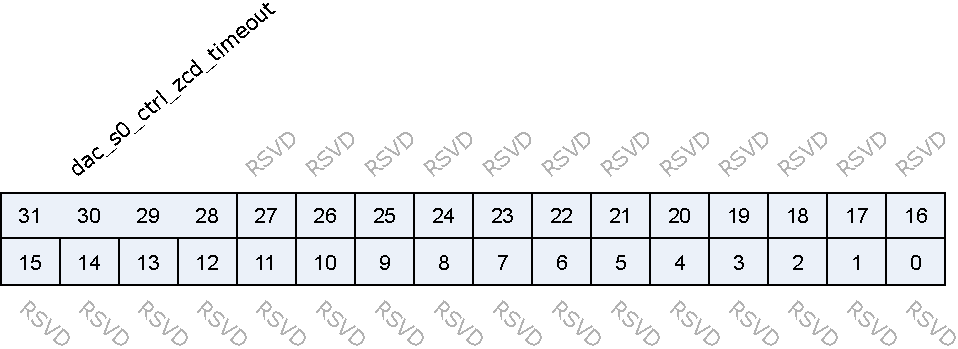
\includegraphics{audac_audac_s0_misc.pdf}
\end{figure}

\regdes{31:28&dac\_s0\_ctrl\_zcd\_timeout&r/w&4'd4&zero crossing time out period \par 0:2 fs sample  \par 1:4 fs sample \par 2:8 fs sample \par 3:16 fs sample \par 4:32 fs sample \par 5:64 fs sample \par 6:128 fs sample \par 7:256 fs sample \par 8:512 fs sample \par 9:1024 fs sample \par 8:2048 fs sample
\\\hline
27:0&RSVD& & & \\\hline

}
\subsection{audac\_zd\_0}
\label{audac-audac-zd-0}
Address:0x20055010
 \begin{figure}[H]
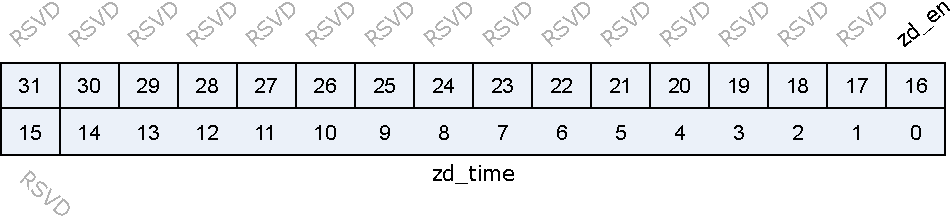
\includegraphics{audac_audac_zd_0.pdf}
\end{figure}

\regdes{31:17&RSVD& & & \\\hline
16&zd\_en&r/w&0&enable zero detect\\\hline
15&RSVD& & & \\\hline
14:0&zd\_time&r/w&15'd512&number of zeros\\\hline

}
\subsection{audac\_1}
\label{audac-audac-1}
Address:0x20055014
 \begin{figure}[H]
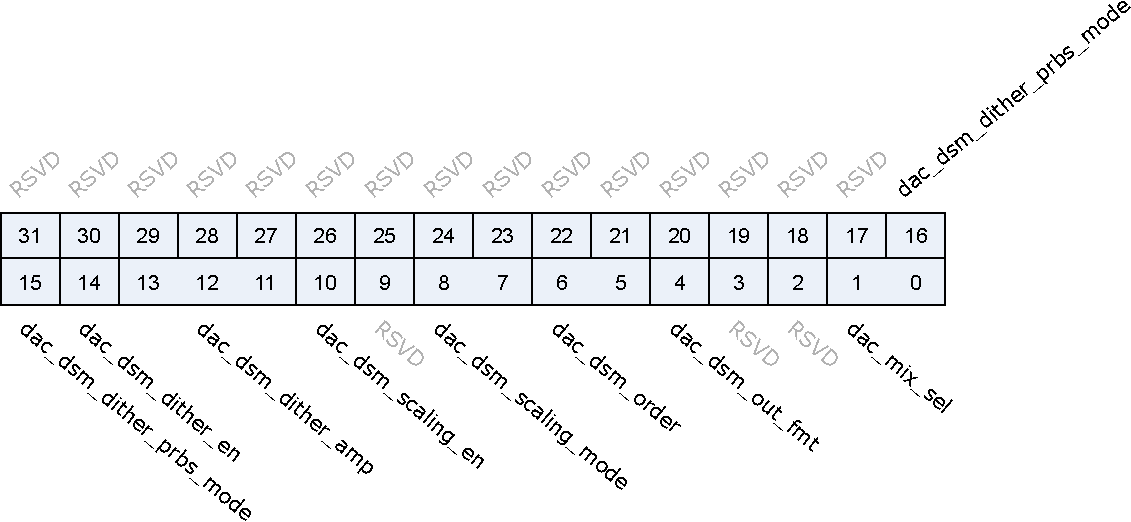
\includegraphics{audac_audac_1.pdf}
\end{figure}

\regdes{31:17&RSVD& & & \\\hline
16:15&dac\_dsm\_dither\_prbs\_mode&r/w&0&dac dsm dither lfsr mode:0:LFSR32, 1:LFSR24, 2:LFSR16, 3:LFSR12\\\hline
14&dac\_dsm\_dither\_en&r/w&1&enable dac dsm dither\\\hline
13:11&dac\_dsm\_dither\_amp&r/w&0&dac dsm dither amplitue\\\hline
10&dac\_dsm\_scaling\_en&r/w&1&enable dac dsm scaling\\\hline
9&RSVD& & & \\\hline
8:7&dac\_dsm\_scaling\_mode&r/w&0&dac dsm scaling value;  u4.4\\\hline
6:5&dac\_dsm\_order&r/w&0&0: 2-order, 1: 3-order\\\hline
4&dac\_dsm\_out\_fmt&r/w&0&offset binary 1:2's complement\\\hline
3:2&RSVD& & & \\\hline
1:0&dac\_mix\_sel&r/w&0&L channel, 1:R channel, 2: L+R, 3: (L+R)/2\\\hline

}
\subsection{audac\_fifo\_ctrl}
\label{audac-audac-fifo-ctrl}
Address:0x2005508c
 \begin{figure}[H]
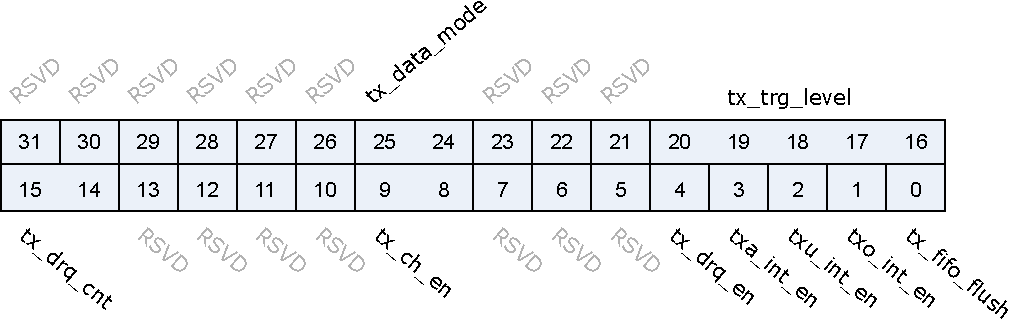
\includegraphics{audac_audac_fifo_ctrl.pdf}
\end{figure}

\regdes{31:26&RSVD& & & \\\hline
25:24&tx\_data\_mode&r/w&2'b0&TX\_FIFO\_DATIN\_MODE. \par TX FIFO DATA Input Mode (Mode 0, 1, 2, 3) \par Mode 0: Valid data's MSB is at [31] of TX\_FIFO register \par Mode 1: Valid data's MSB is at [23] of TX\_FIFO register \par Mode 2: Valid data's MSB is at [19] of TX\_FIFO register \par Mode 3: Valid data's MSB is at [15] of TX\_FIFO register \par For 16-bits transmitted audio sample: \par Mode 0: FIFO\_I[15:0] = {TXDATA[31:16]} \par Mode 1: FIFO\_I[15:0] = {TXDATA[23:8]} \par Mode 2: FIFO\_I[15:0] = {TXDATA[19:4]} \par Mode 3: FIFO\_I[15:0] = {TXDATA[15:0]}
\\\hline
23:21&RSVD& & & \\\hline
20:16&tx\_trg\_level&r/w&5'd7&TX\_FIFO\_TRG\_LEVEL. \par TX FIFO Trigger Level (TXTL[4:0]) \par Interrupt and DMA request trigger level for TX FIFO room available condition \par IRQ/DRQ Generated when WLEVEL > TXTL[4:0] \par Notes: \par WLEVEL represents the number of room available in the TX FIFO
\\\hline
15:14&tx\_drq\_cnt&r/w&2'b0&DAC\_DRQ\_CLR\_CNT. \par When TX FIFO available room less than or equal N, DRQ Request will be de-asserted. N is defined here: \par 00: IRQ/DRQ de-asserted when WLEVEL <= TXTL[4:0] \par 01: IRQ/DRQ de-asserted when WLEVEL < 2 \par 10: IRQ/DRQ de-asserted when WLEVEL < 4 \par 11: IRQ/DRQ de-asserted when WLEVEL < 8 \par WLEVEL represents the number of room available in the TX FIFO
\\\hline
13:10&RSVD& & & \\\hline
9:8&tx\_ch\_en&r/w&2'b0&TX\_FIFO\_DATOUT\_DST. \par TX FIFO Data Output Destination Select. \par 0: Disable 1: Enable \par Bit9: DAC2 data \par Bit8: DAC1 data \par When some of the above bits set to ’1’, these data are always arranged in order from low-bit to high-bit.(bit8->bit9)
\\\hline
7:5&RSVD& & & \\\hline
4&tx\_drq\_en&r/w&1'b0&DAC\_DRQ\_EN. \par DAC FIFO Room Available DRQ Enable. \par 0: Disable \par 1: Enable
\\\hline
3&txa\_int\_en&r/w&1'b0&DAC\_IRQ\_EN. \par DAC FIFO Room Available IRQ Enable. \par 0: Disable \par 1: Enable
\\\hline
2&txu\_int\_en&r/w&1'b0&DAC\_UNDERRUN\_IRQ\_EN. \par DAC FIFO Under Run IRQ Enable \par 0: Disable \par 1: Enable
\\\hline
1&txo\_int\_en&r/w&1'b0&DAC\_OVERRUN\_IRQ\_EN. \par DAC FIFO Over Run IRQ Enable \par 0: Disable \par 1: Enable
\\\hline
0&tx\_fifo\_flush&w1c&1'b0&DAC\_FIFO\_FLUSH. \par DAC FIFO Flush. \par Write ‘1’ to flush TX FIFO, self clear to ‘0’.
\\\hline

}
\subsection{audac\_fifo\_status}
\label{audac-audac-fifo-status}
Address:0x20055090
 \begin{figure}[H]
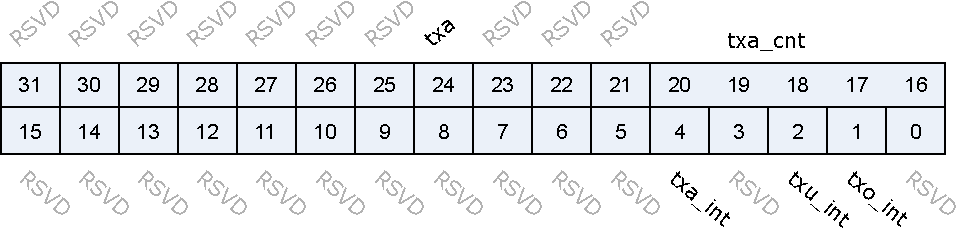
\includegraphics{audac_audac_fifo_status.pdf}
\end{figure}

\regdes{31:25&RSVD& & & \\\hline
24&txa&r&1'b1&TXA. \par TX FIFO Room Available \par 0: No room for new sample in TX FIFO \par 1: More than one room for new sample in TX FIFO (>= 1 word)
\\\hline
23:21&RSVD& & & \\\hline
20:16&txa\_cnt&r&5'd16&TXA\_CNT. \par TX FIFO Available Room Word Counter
\\\hline
15:5&RSVD& & & \\\hline
4&txa\_int&r&1'b0&TXA\_INT. \par TX FIFO Room Available Pending Interrupt \par 0: No Pending IRQ \par 1: Room Available Pending IRQ \par Automatic clear if interrupt condition fails.
\\\hline
3&RSVD& & & \\\hline
2&txu\_int&r&1'b0&TXU\_INT. \par TX FIFO Underrun Pending Interrupt \par 0: No Pending IRQ \par 1: FIFO Underrun Pending IRQ \par Write ‘1’ to clear this interrupt
\\\hline
1&txo\_int&r&1'b0&TXO\_INT. \par TX FIFO Overrun Pending Interrupt \par 0: No Pending IRQ \par 1: FIFO Overrun Pending IRQ \par Write ‘1’ to clear this interrupt
\\\hline
0&RSVD& & & \\\hline

}
\subsection{audac\_fifo\_data}
\label{audac-audac-fifo-data}
Address:0x20055094
 \begin{figure}[H]
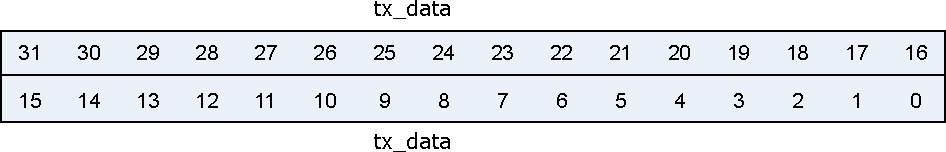
\includegraphics{audac_audac_fifo_data.pdf}
\end{figure}

\regdes{31:0&tx\_data&w&32'h0&TX\_DATA. \par Transmitting left, right channel sample data should be written this register one by one. The left channel sample data is first and then the right channel sample.
\\\hline

}
